\chapter{Model of the Mobile Manipulator}
\label{chapter2}

\section{Mobile Robot Model}
\subsection{Kinematics}
Assuming to have a $n$ dimensional, $k$ constraint equations imply that the admissible generalized velocities of the system for any of its configurations q necessarily belong to a $(n-k)$-dimensional space. Specifically, expressing the constraint equations in Pfaffian form, the generalized velocities should belong to the null space of matrix $A^T$.\\
Thus, it can be written:
\begin{equation} \label{G}
\dot{q}=\sum_{j=1}^{m} g_j(q)u_j=G(q)u \qquad m=n-k
\end{equation}
Where $q\in \mathbb{R}^n $ is the state vector, $u= \left[
\begin{matrix}
u_1 &  \cdots & u_m
\end{matrix}
\right]^T\in\mathbb{R}^m $ is the input vector and $\left\lbrace  g_1 (q) \cdots g_m (q) \right\rbrace $ is a basis of the null space of $A^T$, named \textit{input vector fields}. \\
The choice of the input vector fields is not unique, since the input u can have different meanings: velocities, torques or others.

\subsubsection{Unicycle Model}
\begin{figure}[h!]
	\centering
	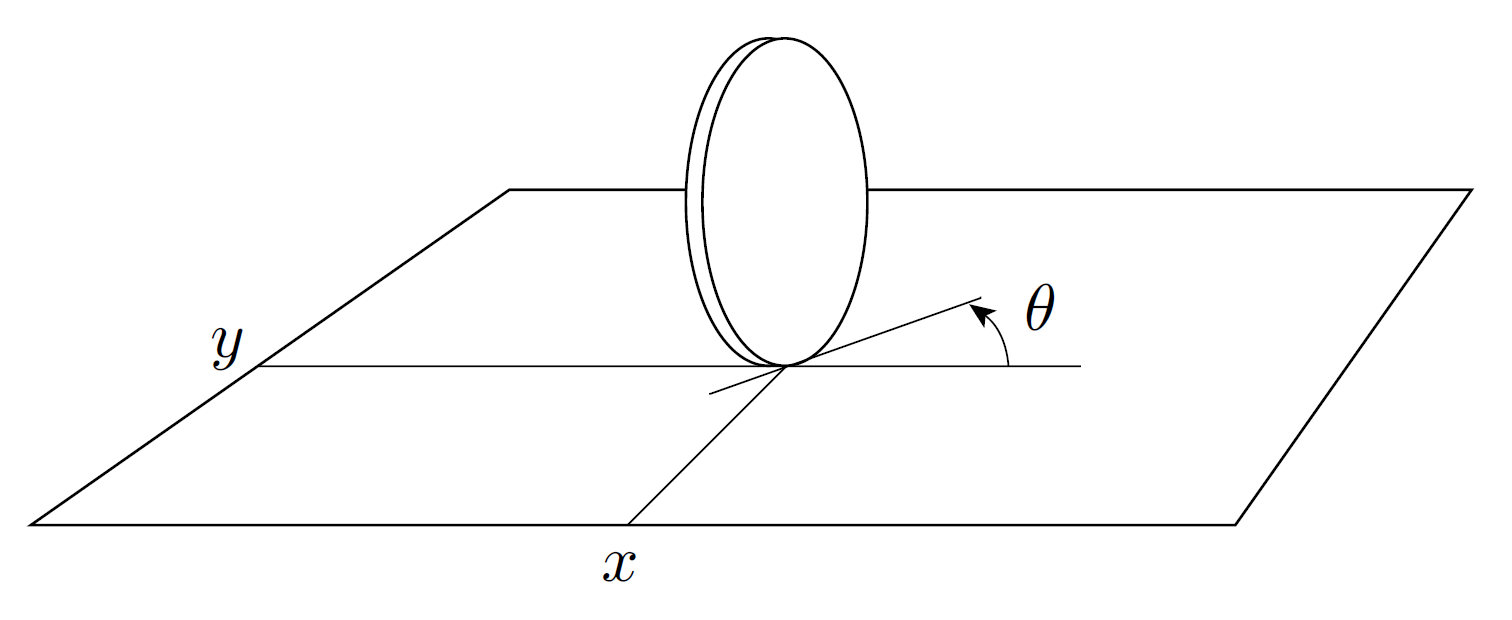
\includegraphics[scale=0.4]{unicycle_model}
	\caption{Unicycle model}
\end{figure}
A unicycle is a vehicle which configuration is completely described by the state vector $q = [x y \theta]^T$, where $x$ and $y$ are the Cartesian coordinates of the contact point of the wheel with the ground or of the wheel centre and $\theta$ is the orientation of the wheel with respect to the $x$ axis. \\
As we already seen in the previous chapter, the constraint of pure rolling for the unicycle is expressed as:
\begin{equation} 
\dot{x}\sin\theta-\dot{y}\cos\theta=\left[
\begin{matrix}
\sin\theta & cos\theta & 0
\end{matrix}
\right] \dot{q}=0
\end{equation}
\begin{equation*} \label{At}
A^T \left( q \right)\dot{q} =0  
\end{equation*}
This equation expresses that the velocity of the contact point (or of the wheel centre) is zero in the direction orthogonal to the sagittal axis of the disk.\\
Hence in the unicycle case $n=3$ and $k=1$, so the dimension of the basis of the null space of $A^T$ is 2. Choosing:
\begin{equation} 
G(q)=\left[
\begin{matrix}
g_1 (q) & g_2 (q)
\end{matrix}
\right] =  \left[
\begin{matrix}
\cos\theta & 0 \\
\sin\theta & 0 \\
0 & 1 
\end{matrix}
\right]
\end{equation}
All the generalized velocities of the unicycle at q are a combination of $g_1 (q)$ and $g_2 (q)$.
\begin{equation} 
\dot{q}=\left[
\begin{matrix}
\dot{x} \\ \dot{y} \\\dot{\theta}
\end{matrix}
\right] =  \left[
\begin{matrix}
\cos\theta \\ \sin\theta \\ 0 
\end{matrix}
\right]v + \left[
\begin{matrix}
0 \\ 0 \\ 1 
\end{matrix}
\right]\omega
\end{equation}
Where $v$ is the driving velocity, i.e. the velocity of the disk along its sagittal plane, and $\omega$ is the steering velocity, i.e. the angular speed around its vertical axis.\\
A lot of mobile robots are kinematically equivalent to a unicycle, like differential drive robots, skid steering robots or synchro drive vehicles.\\
In most of the unicycle-like mobile robots, $v$ and $\omega$ are the command input to the system, while the actual velocity input are $\omega_R$ and $\omega_L$, i.e. the right and left wheels angular speeds. 
\begin{equation}
v=\frac{r\left(\omega_R + \omega_L\right)}{2} \qquad \omega=\frac{r\left(\omega_R - \omega_L\right)}{d}
\end{equation}
\begin{equation}
\omega_R =\frac{1}{r}\left(v+\frac{d}{2}\omega\right) \qquad \omega_L=\frac{1}{r}\left(v-\frac{d}{2}\omega\right)
\end{equation}
Where $r$ is the wheels radius and $d$ is the distance between their centres.

\subsubsection{Bicycle Model}
\begin{figure}[h!]
	\centering
	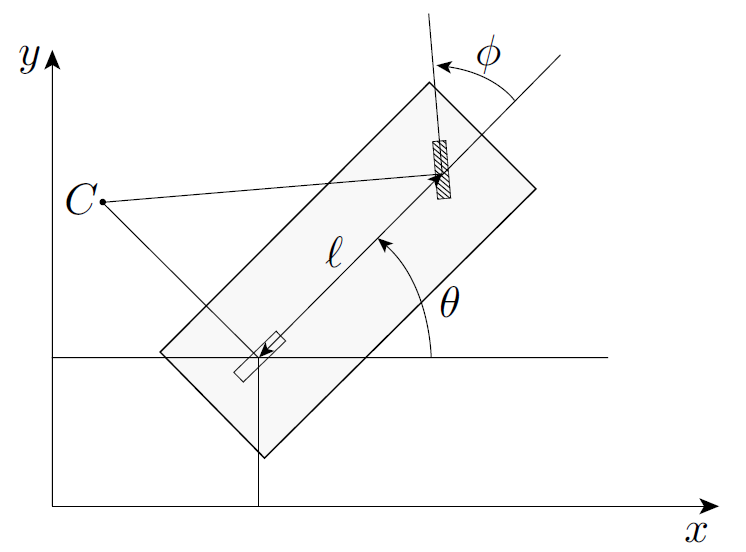
\includegraphics[scale=0.7]{bicycle_model}
	\caption{Bicycle model}
\end{figure}
A bicycle is a vehicle having an orientable wheel and a fixed wheel. Kinematically it can be described with the generalized coordinates $q = [x y \theta \phi]^T$ , where $x$ and $y$ are the Cartesian coordinates of the centre of the rear wheel, $\theta$ is the orientation of the vehicle with respect to the $x$ axis, and $\phi$ is the steering angle of the front wheel with respect to the vehicle axis.\\
Both wheels are subject to pure rolling constraints. So expressing the zero velocity of the centre of the front wheel in the direction orthogonal to the wheel itself, and the zero velocity of the centre of the rear wheel in the direction orthogonal to the sagittal axis of the vehicle:
\begin{equation}
\dot{x}_f\sin \left( \theta+\phi \right)-\dot{y}_f \cos\left(\theta+\phi\right)=0
\end{equation}
\begin{equation}
\dot{x}\sin\theta-\dot{y}\cos\theta=0
\end{equation}
Where:
\begin{align*}
x_f=x+\ell\cos\theta \\
y_f=y+\ell\sin\theta
\end{align*}
Are the cartesian coordinates of the centre of the front wheel.\\
The lines orthogonal to the two wheels meet in the instantaneous centre of rotation $C$.\\
The pure rolling constraints written in the above equation can be expressend in the Pfaffian form as:
\begin{equation*} 
A^T \left( q \right)\dot{q} =0  
\end{equation*}
\begin{equation}
A^T \left( q \right) = \left[ 
\begin{matrix}
\sin\theta & -\cos\theta & 0 & 0 \\
\sin\left(\theta+\phi \right) & -\cos\left(\theta+\phi \right) & -\ell\cos\phi & 0
\end{matrix}
\right]
\end{equation}
Following the same reasoning done before, we have 4 degrees of freedom and 2 kinematic constraints, so the dimension of the null space of $A(q)^T$ is $n-k= 2$. An example of basis of the null space is:
\begin{equation}
\left[ 
\begin{matrix}
\dot{x} \\ 	\dot{y} \\ 	\dot{\theta} \\	\dot{\phi} 
\end{matrix}
\right] = \left[
\begin{matrix}
\cos\theta\cos\phi \\ \sin\theta\cos\phi \\ \sin\phi/\ell \\ 0 
\end{matrix}
\right] v+ \left[
\begin{matrix}
0 \\0 \\0 \\1
\end{matrix}
\right] \omega
\end{equation}
If the vehicle is front-wheel drive, or:
\begin{equation}
\left[ 
\begin{matrix}
\dot{x} \\ 	\dot{y} \\ 	\dot{\theta} \\	\dot{\phi} 
\end{matrix}
\right] = \left[
\begin{matrix}
\cos\theta \\ \sin\theta \\ \tan\phi/\ell \\ 0 
\end{matrix}
\right] v+ \left[
\begin{matrix}
0 \\0 \\0 \\1
\end{matrix}
\right] \omega
\end{equation}
If the vehicle is rear-wheel drive.

\subsection{Dynamics}
The dynamic model of a mobile robot can be derived using the Lagrangian formulation for a $n$-dimensional system, defining the Lagrangian $L$ of the mechanical system as the difference between kinetic and potential energy.
\begin{equation}
\mathcal{L}(q,\dot{q})=\mathcal{T}(q,\dot{q})-\mathcal{U}(q)=\frac{1}{2}\dot{q}^T B(q)\dot{q} - \mathcal{U}(q)
\end{equation}
Where $B(q)$ is the inertia matrix, which is symmetric and positive definite.\\
Writing the Lagrange equations:
\begin{equation}
\frac{d}{dt}\left(\frac{\partial\mathcal{L}}{\partial\dot{q}} \right) - \left(\frac{\partial\mathcal{L}}{\partial q} \right)^T=S(q)\tau+A(q)\lambda
\end{equation}
In this formulation we are adding the energetical term due to the kinematic constraints adding the \textit{Lagrange multipliers} term. 
Substituting the Lagrangian term, we obtain the dynamic model of the mobile base:
\begin{equation}
B(q)\ddot{q}+C(q,\dot{q})\dot{q}+g(q) = S(q)\tau+A(q)\lambda
\end{equation}
\begin{equation*} 
A^T \left( q \right)\dot{q} =0  
\end{equation*}
Where:
\begin{equation}
C(q,\dot{q})=\dot{B}(q)\dot{q}-\frac{1}{2}\left(\frac{\partial}{\partial q}\left( \dot{q}^T B(q)\dot{q}\right)\right)^T
\end{equation}
\begin{equation}
g(q) = \frac{\partial\mathcal{U}(q)}{\partial q} = 0
\end{equation}
The potential energy of a mobile base during its motion can be considered constant, so it is possible to disregard it.\\
It is possible to further simplify the dynamic model exploiting a useful property of the kinematic relation \ref{G}. Since we defined the coloums of $G(q)$ as vectors belonging to the null space of $A(q)^T$, the following relation holds:
\begin{equation}
A(q)^T G(q) = 0 \qquad\textrm{or}\qquad G(q)^T A(q) = 0
\end{equation}
So, premultiplying the dynamic model by $G(q)^T$:
\begin{equation}
G^T(q)\left(B(q)\ddot{q}+C(q,\dot{q})\dot{q}\right) = G^T(q)S(q)\tau
\end{equation}
Reducing the $n$ differential equations to a system of $m$ differential equations without Lagrange multipliers.
\subsubsection{Unicycle Model}
\begin{figure}[h!]
	\centering
	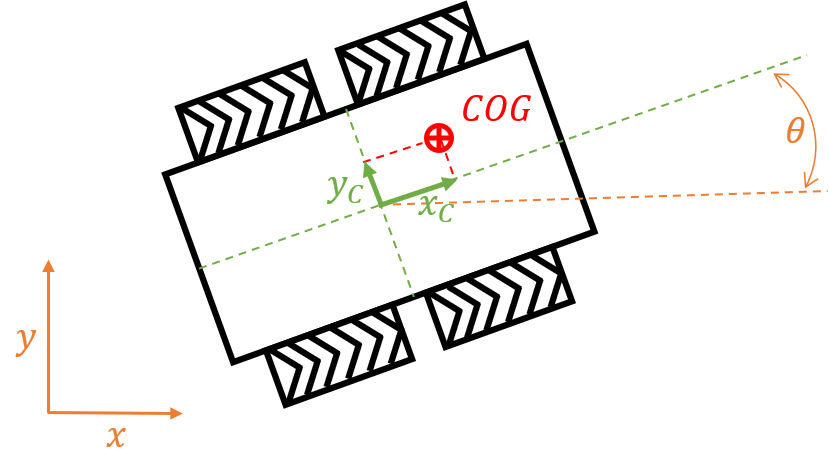
\includegraphics[scale=0.7]{schema_mobile_base}
	\caption{Scheme of a Differential Drive Mobile Robot}
	\label{diffdrive}
\end{figure}
In a unicycle case, like a differential drive robot (Figure \ref{diffdrive}), the kinetic energy can be expressed as: 
\begin{equation}
\mathcal{T}(q,\dot{q})=\frac{1}{2}M\dot{x}_{COG}^2 + \frac{1}{2}M\dot{y}_{COG}^2 + \frac{1}{2}J\dot{\theta}^2
\end{equation}
Where:
\begin{align*}
x_{COG} = x+x_C\cos\theta-y_C\sin\theta\\ 
y_{COG} = y+x_C\sin\theta+y_C\cos\theta
\end{align*}
Are the global coordinates of the centre of gravity of the mobile base, and their velocities are:
\begin{align*}
\dot{x}_{COG} = \dot{x}-\dot{\theta}x_C\sin\theta-\dot{\theta}y_C\cos\theta\\ 
\dot{y}_{COG} = \dot{y}+\dot{\theta}x_C\cos\theta-\dot{\theta}y_C\sin\theta
\end{align*}
And $M$ and $J$ are respectively the base’s mass and moment of inertia along its vertical axis $z$.\\
So, after substituting these equations in the Lagrange equation we can write:
\begin{equation*}
B(q)=\left[ 
\begin{matrix}
M & 0 & -M\left( x_C\sin\theta + y_C\cos\theta\right) \\
0 & M & M\left( x_C\cos\theta - y_C\sin\theta\right) \\
-M\left( x_C\sin\theta + y_C\cos\theta\right) & M\left( x_C\cos\theta - y_C\sin\theta\right) & J+M x_C^2+M y_C^2
\end{matrix}
\right]
\end{equation*}
\begin{equation}
C(q,\dot{q})=\left[ 
\begin{matrix}
0 & 0 & M\dot{\theta}\left( y_C\sin\theta - x_C\cos\theta\right) \\
0 & 0 & -M\dot{\theta}\left( y_C\cos\theta +x_C\sin\theta\right) \\
0 & 0 & 0
\end{matrix}
\right]
\end{equation}
Taking the kinematic equation of the unicycle model, deriving it and substituting it in the reduced dynamic model we obtain:
\begin{equation}
\dot{q}=G(q)\left[
\begin{matrix}
v_{long} \\ \omega
\end{matrix}
\right] =G(q)v
\end{equation}
\begin{equation}
\ddot{q}=\dot{G}(q)v+G(q)\dot{v}
\quad
\end{equation}
\begin{equation}
\tilde{B}(q)\dot{v}+\tilde{C}(q,\dot{q})v = \tilde{S}(q)\tau
\end{equation}
Where:
\begin{align*}
&\tilde{B}(q) = G^T(q)B(q)G(q) \\
&\tilde{C}(q,\dot{q}) = G^T(q)C(q,\dot{q})G(q) + G^T(q)B(q)\dot{G(q)} \\
&\tilde{S}(q) = G^T(q)S(q) 
\end{align*}
In this way it is also possible to express the system in \textit{state space form}:
\begin{equation}
\left[ 
\begin{matrix}
\dot{q} \\ \dot{v}
\end{matrix}
\right] = \left[ 
\begin{matrix}
[0] & G(q)\\ [0] & -\tilde{B}^{-1}\tilde{C}
\end{matrix}
\right]\left[ 
\begin{matrix}
q \\ v
\end{matrix}
\right] + \left[ 
\begin{matrix}
[0] \\ \tilde{B}^{-1}\tilde{S}
\end{matrix}
\right] \tau
\end{equation}
All the system can be eventually simplified considering the centre of gravity in the geometric centre of the mobile robot. 
\begin{equation*}
x_C=0\quad,\quad y_C=0;
\end{equation*}
\begin{equation}
B(q) = \left[\begin{matrix}
M & 0 & 0\\ 0 & M & 0 \\ 0 & 0 & J
\end{matrix} \right]
\qquad 
C(q,\dot{q}) = \left[\begin{matrix}
0 & 0 & 0\\ 0 & 0 & 0 \\ 0 & 0 & 0
\end{matrix} \right]
\end{equation}
\begin{equation}
\tilde{B}(q)\dot{v} = \tilde{S}(q)\tau
\end{equation}
So, the state space dynamic model becomes:
\begin{equation}
\left[ 
\begin{matrix}
\dot{q} \\ \dot{v}
\end{matrix}
\right] = \left[ 
\begin{matrix}
[0] & G(q)\\ [0] & [0]
\end{matrix}
\right]\left[ 
\begin{matrix}
q \\ v
\end{matrix}
\right] + \left[ 
\begin{matrix}
[0] \\ \tilde{B}^{-1}\tilde{S}
\end{matrix}
\right] \tau
\end{equation}

\section{Manipulator Model}
\subsection{Kinematics}
A manipulator consists of a series of rigid links connected by joints. In order to plan the manipulator motion from an initial to a final configuration, i.e. the set of joint values, it is necessary to define its pose with respect to a reference frame. 
\subsubsection{Rototraslation Matrices}
An orthonormal reference frame $\textbf{x’,y’,z’}$ can be described with respect to an orthonormal reference frame $\textbf{x,y,z}$ in the following way:
\begin{align}
\textbf{x'}=x'_x\textbf{x}+x'_y\textbf{y}+x'_z\textbf{z}\\
\textbf{y'}=y'_x\textbf{x}+y'_y\textbf{y}+y'_z\textbf{z}\\
\textbf{z'}=z'_x\textbf{x}+z'_y\textbf{y}+z'_z\textbf{z}
\end{align}
\begin{figure}[h!]
	\centering
	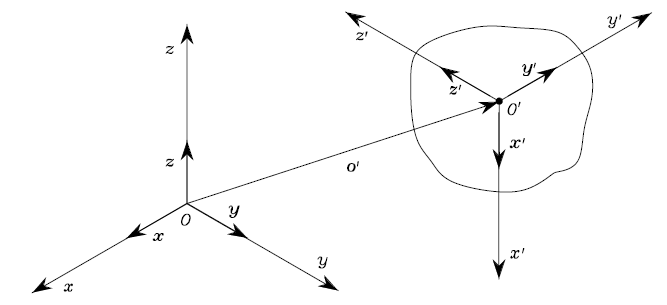
\includegraphics[scale=1]{rotation_frames}
	\caption{}
\end{figure}
These three equations can be expressed as a rotation matrix of the frame $\textbf{x’,y’,z’}$ with respect to the frame $\textbf{x,y,z}$:
\begin{equation}
R= \left[
\begin{matrix}
\textbf{x'} & \textbf{y'} & \textbf{z'}
\end{matrix}
\right]=\left[
\begin{matrix}
x'_x & y'_x & z'_x \\
x'_y & y'_y & z'_y \\
x'_z & y'_z & z'_z 
\end{matrix}
\right] 	
\end{equation}
Consider now a point P whose coordinates are referred to frame $\textbf{x,y,z}$ describe the vector $\textbf{p}$, and the coordinates referred to the rotated frame $\textbf{x’,y’,z’}$ describe the vector $\textbf{p’}$. Then it is possible to write:
\begin{equation}
	\textbf{p} = \left[
	\begin{matrix}
		p_x \\ p_y \\ p_z
	\end{matrix}
	\right]
	\quad
	\textbf{p'} = \left[
	\begin{matrix}
		p'_x \\ p'_y \\ p'_z
	\end{matrix}
	\right]
\end{equation}
\begin{equation}
	\textbf{p} = p'_x\textbf{x'}+p'_y\textbf{y'}+p'_z\textbf{z'}=\left[
	\begin{matrix}
		\textbf{x'} & \textbf{y'} & \textbf{z'}
	\end{matrix}
	\right] \textbf{p'} = R \textbf{p'}
\end{equation}
\begin{figure}[h!]
	\centering
	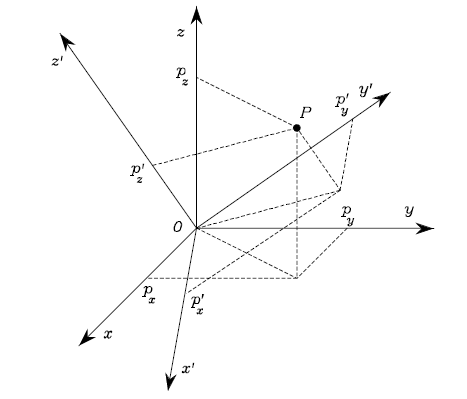
\includegraphics[scale=1]{rotation_frames1}
	\caption{}
\end{figure}
The rotation matrix is orthogonal because its columns are mutually orthogonal, by definition.
\begin{equation}
	R^TR=I \qquad R^T=R^{-1}
\end{equation}
If we then consider two different reference frames: $x^0,y^0,z^0$ and $x^1,y^1,z^1$ with two different origins $O^0$ and $O^1$, a point P is represented by the two frames respectively with vectors $p^0$ and $p^1$.
\begin{figure}[h!]
	\centering
	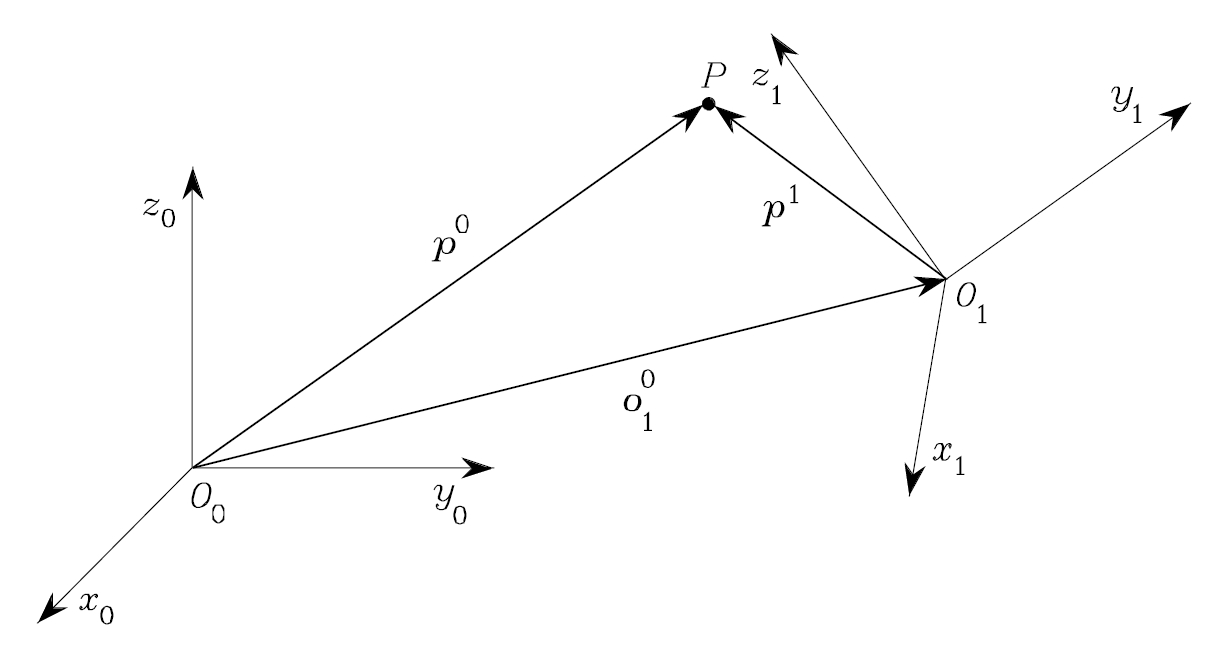
\includegraphics[scale=1.3]{rototraslation_frames}
	\caption{}
\end{figure}
The vector $p^0$ can be represented as the sum of two vectors:
\begin{equation} \label{rototrasl}
	\mathbf{p^0}= \mathbf{o_1^0} + R_1^0 \mathbf{p^1}
\end{equation}
Where $R^0_1$ is the rotation matrix of frame $x^1,y^1,z^1$ with respect to frame $x^0,y^0,z^0$ and so $R_1^0 \mathbf{p^1}$ is the representation of vector $\mathbf{p^1}$ in the frame $x^0,y^0,z^0$.\\
It is possible to express the equation above in a compact form using the homogenous transformation matrix simply defining:
\begin{equation} \label{A}
	\tilde{\mathbf{p}}=\left[
	\begin{matrix}
	\textbf{p} \\ 1
	\end{matrix}
	\right] \qquad 
	A_1^0 = \left[
	\begin{matrix}
       R_1^0 & \mathbf{o_1^0} \\ [0] & 1
	\end{matrix}
	\right]
\end{equation}
\begin{equation}
	\tilde{\mathbf{p}}^0 = A_1^0\tilde{\mathbf{p}}^1
\end{equation}
The matrix $A_1^0$ is called \textit{rototraslation matrix}.\\
Inverting the equation \ref{rototrasl} we can express the inverse transformation.
\begin{equation} 
\mathbf{p^1}= -R_0^1\mathbf{o_1^0} + R_0^1 \mathbf{p^0}
\end{equation}
\begin{equation}
	A_0^1 = \left[
	\begin{matrix}
		R_0^1 & -R_0^1\mathbf{o_1^0} \\ [0] & 1
	\end{matrix}
	\right]
\end{equation}
Where:
\begin{equation*}	
	R_0^1 = (R_1^0)^{-1}=(R_1^0)^{T}
\end{equation*}
\begin{equation*}
A_0^1 = (R_1^0)^{-1}
\end{equation*}
Both with rotation and rototraslation matrices, it is possible to obtain a composition of consecutive transformations by postmultiplying the matrices related to the single rotations:
\begin{align}
	R_2^0 = R_1^0R_2^1\\
	A_2^0 = A_1^0A_2^1	
\end{align}

\subsubsection{Denavit-Hartenberg Parameters}
Since the first ‘80s a popular approach to describe the kinematics of robots, and therefore the rototraslation matrices to express the transformation from one joint frame to the following, is the convention introduced by Jacques Denavit and Richard Hartenberg in 1955 for a compact description of mechanisms.  
Their representation is based on the concept of the common normal between joint axes, defined as the shortest line between two axes, perpendicular to both axes. 

\begin{figure}[h!]
	\centering
	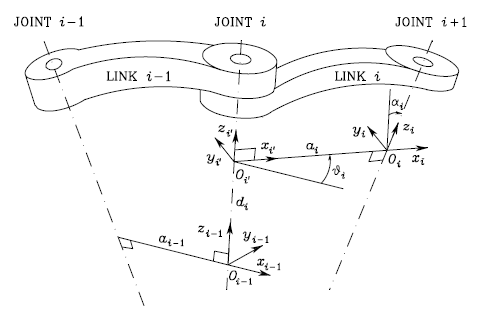
\includegraphics[scale=1.3]{denavit_hartenberg}
	\caption{Denavit-Hartenberg convention for Robot links}
\end{figure}

The convention firstly assigns to each link a reference frame referring to the following rules: 
\begin{itemize}
	\item Axis $z_i$ is chosen along the axis of joint i+1;
	\item The origin $O_i$ is located at the intersection of axis $z_i$ with the common normal to axes $z_{i-1}$ and $z_i$;
	\item Axis $x_i$ is chosen as an extension of the common normal to axes $z_{i-1}$ and $z_i$;
	\item Axis $y_i$ is chosen to complete a right-handed frame.
\end{itemize}
Once established a frame for each link, 4 parameters describe the pose of frame i with respect to frame i-1.
\begin{itemize}
	\item $a_i$ : distance between $z_i$ and $z_{i-1}$. Only geometrical, depends only on the geometry of the links
	\item $d_i$ : coordinate of $O_i$ along $z_{i-1}$. Varies if the joint is prismatic.
	\item $\alpha_i$: angle between axes $z_{i-1}$ and $z_i$ (positive counterclockwise with respect to axis $x_i$). Only geometrical, depends only on the geometry of the links.
	\item $\theta_i$: angle between axes $x_{i-1}$ and $x_i$ (positive counterclockwise with respect to axis $z_{i-1}$). Varies if the joint is revolute.
\end{itemize}
The transformation matrix between frame i and frame i-1 can then be built:
\begin{equation}
	A_i^{i-1}(q_i)=\left[
	\begin{matrix}
		\cos\theta & -\sin\theta\cos\alpha & \sin\theta\sin\alpha & a\cos\theta \\
		\sin\theta & \cos\theta\cos\alpha & -\cos\theta\sin\alpha & a\sin\theta \\
		0 & \sin\alpha & \cos\alpha & d \\
		0 & 0 & 0 & 1
	\end{matrix}
	\right]
\end{equation}
This matrix is function only on the joint variables $\theta$ and $d$.

\subsubsection{Direct and Inverse Kinematics} \label{dirinvkin}
As anticipated, a manipulator is basically made of links chained together by joints that connect the \textit{base} of the manipulator to its \textit{end effector}.\\
The \textit{direct kinematics} of the manipulator express the position and orientation of the end effector as a function of the robot configuration. Using the concepts showed up to this point, this corresponds to the definition of the rototraslation matrix that describes the end effector frame with respect to the global reference frame:
\begin{equation}\label{AAAA}
	A_{ee}^{base}=A_1^{base}A_2^1A_3^2\cdots A_{ee}^{ee-1}
\end{equation}
The opposite problem is the definition of the \textit{inverse kinematics}, i.e. given the position and orientation of the end effector, finding the corresponding joint variables. The inverse kinematics problem is not easy to solve since it is often nonlinear and there can be infinite solutions as well as none.\\
An important concept which roboticists are still working on is \textit{kinematic redundancy}, i.e. when the number of joint variables is greater than the dimension of the operational space, which is 6 in case of the definition of the 3D position and orientation of the end effector. 
When a system is kinematically redundant, direct kinematics is always possible to be defined, while inverse kinematics can have infinite solutions.
Solving the \textit{kinematic redundancy problem} means to define a criterion in order to be able to pick one among the infinite configurations which have the end effector in the same position and orientation.\\
This concept will be very important in the defintion of Mobile Manipulator control.
\subsection{Dynamics}
\label{sec:dynamics}
As we already seen in the case of mobile robots the dynamics of a robot can be expressed with the Euler-Lagrange formulation.
\begin{equation*}
	\mathcal{L}=\mathcal{T}-\mathcal{U}
\end{equation*}
\begin{equation*}
	\frac{d}{dt}\left(\frac{\partial\mathcal{L}}{\partial\dot{q}} \right) - \left(\frac{\partial\mathcal{L}}{\partial q} \right)^T=\tau
\end{equation*}
Where $q$ is the vector of the generalized coordinates and $\tau$ is the vector of the generalized forces.\\
The potential energy of the manipulator is given by
\begin{equation}
	\mathcal{U} = \sum_{i=1}^{n}\left(\mathcal{U}_{l_i}+\mathcal{U}_{m_i}\right)
\end{equation}
Where $\mathcal{U}_{l_i}$ and $\mathcal{U}_{m_i}$ are the potential energy due to the gravitational forces of the links and of the motors respectively.\\
Similarly, the kinetic energy of the entire system is the sum of the kinetic energies of the links and of the motors 
\begin{equation}
	\mathcal{T} = \sum_{i=1}^{n}\left(\mathcal{T}_{l_i}+\mathcal{T}_{m_i}\right)
\end{equation}
Beginning with the expression of the links kinetic energy:
\begin{equation}
	\mathcal{T}_{l_i}=\frac{1}{2}\int_{V_{l_i}}\dot{\mathbf{p}*}_i^T\dot{\mathbf{p}*}_i\rho dV
\end{equation}
Where $\dot{\mathbf{p}*}_i$ the velocity vector of the elementary particle of link i.\\
In order to relate the velocities of every elementary particle of the manipulator to the joint velocities we have to express in a proper way the Jacobians.

\subsubsection{Differential Kinematics}
First of all we need to introduce the skew symmetric matrix $S(\boldsymbol{\omega})$. It can be obtained from the differentiation with respect to time of a rotation matrix:
\begin{equation}
	R(t)R(t)^T=I
\end{equation}
\begin{equation}
	\dot{R}(t)R(t)^T+R(t)\dot{R}(t)^T=0
\end{equation}
$S$ is defined as:
\begin{equation}
	S(t) = \dot{R}(t)R(t)^T
\end{equation}
It is possible now to define the derivative of the rotation matrix as:
\begin{equation}
	\dot{R}\left(t\right)=S\left(t\right)R(t)
\end{equation}
\begin{equation}
	p\left(t\right)=R\left(t\right)p'
\end{equation}
\begin{equation}
	\dot{p}\left(t\right)=\dot{R}\left(t\right)p'=S(t)R\left(t\right)p'
\end{equation}
But from mechanics it is also known that:
\begin{equation}
	\dot{p}\left(t\right)=\boldsymbol{\omega}(t)\times R\left(t\right)p'
\end{equation}
Where $\boldsymbol{\omega}\left(t\right)=\left[\begin{matrix}\omega_x&\omega_y&\omega_z\end{matrix}\right]$ is the vector of the angular velocity of the rotating frame described by $R(t)$.
So $S$ can be interpreted as an operator depending only on $\boldsymbol{\omega}\left(t\right)$.
\begin{equation}
	S\left(\boldsymbol{\omega}\right)=\left[
	\begin{matrix}
	0&-\omega_z&\omega_y\\\omega_z&0&-\omega_x\\-\omega_y&{-\omega}_x&0
	\end{matrix}\right]
\end{equation}

\subsubsection{Jacobians}\label{jacobians}
In order to express the Lagrange equation as a function of the joint variables velocities we now introduce the Jacobian matrices for each link.
\begin{align}
	{\dot{\mathbf{p}}}_{l_i}=\mathit{j}_{P_1}^{(l_i)}{\dot{q}}_1+\mathit{j}_{P_2}^{(l_i)}{\dot{q}}_2+\cdots+\mathit{j}_{P_i}^{\left(l_i\right)}{\dot{q}}_i=\mathcal{J}_P^{(l_i)}\dot{q}
	\\
	\omega_{l_i}=\mathit{j}_{O_1}^{(l_i)}{\dot{q}}_1+\mathit{j}_{O_2}^{(l_i)}{\dot{q}}_2\cdots+\mathit{j}_{O_i}^{\left(l_i\right)}{\dot{q}}_i=\mathcal{J}_O^{(l_i)}\dot{q}
\end{align}

Where with $\mathcal{J}_P^{(l_i)}$ we mean the Jacobian matrix relating the joint velocities to the linear velocity of the centre of mass of link i, and with $\mathcal{J}_O^{(l_i)}$ we mean the Jacobian matrix relating the joint velocities to the angular velocity of the centre of mass of link i. 
The columns of the Jacobian matrices are:
\begin{equation}
	\mathit{j}_{P_j}^{(l_i)}=
	\begin{cases}
		z_{j-1} & \text{for a \textit{prismatic} joint} \\
		z_{j-1}\times \left(\mathbf{p}_{l_i}-\mathbf{p}_{j-1}\right) & \text{for a \textit{revolute} joint}	
	\end{cases}                                             
\end{equation}
\begin{equation}
	\mathit{j}_{O_j}^{(l_i)}= 
	\begin{cases}
		0 & \text{for a \textit{prismatic} joint} \\
		z_{j-1} & \text{for a \textit{revolute} joint}	
	\end{cases} 
\end{equation}

\subsubsection{Inertia Matrix}
Recovering the kinetic energy expression, we can now relate the velocities $ {\dot{\mathbf{p}*}}_i$ to the velocity vector ${\dot{\mathbf{p}}}_{l_i}$ of the centre of mass of the link.
\begin{equation}
	{\dot{\mathbf{p}*}}_i={\dot{\mathbf{p}}}_{l_i}+\boldsymbol{\omega}_i\times\mathbf{r}_i={\dot{\mathbf{p}}}_{l_i}+S(\boldsymbol{\omega}_i)\mathbf{r}_i
\end{equation}
Substituting this expression in the equation of the kinetic energy and exploiting the properties of the integral of the centre of mass we obtain.
\begin{equation}
	\mathcal{T}_{l_i}= \frac{1}{2}m_{l_i}{{\dot{\mathbf{p}}}_{l_i}}^T{\dot{\mathbf{p}}}_{l_i}+\frac{1}{2}{\boldsymbol{\omega}_i}^TR_iI_{l_i}^iR_i^T\boldsymbol{\omega}_i
\end{equation}
\begin{equation}
	\mathcal{T}_{l_i}= \frac{1}{2}m_{l_i}{\dot{q}}^T{\mathcal{J}_P^{(l_i)}}^T\mathcal{J}_P^{(l_i)}\dot{q}+\frac{1}{2}{\dot{q}}^T{\mathcal{J}_O^{(l_i)}}^TR_iI_{l_i}^iR_i^T\mathcal{J}_O^{(l_i)}\dot{q}
\end{equation}

In an analogous way it can be computed also the motors kinetic energy.
\begin{equation}
	\mathcal{T}_{m_i}=
	\frac{1}{2}m_{m_i}{{\dot{\mathbf{p}}}_{m_i}}^T{\dot{\mathbf{p}}}_{m_i}+\frac{1}{2}{\boldsymbol{\omega}_{m_i}}^TI_{m_i}\boldsymbol{\omega}_{m_i}
\end{equation}

Where ${\dot{\mathbf{p}}}_{m_i}$ is the velocity vector of the centre of mass of the motor and $\boldsymbol{\omega}_{m_i}$ is the angular velocity of the rotor of motor i.
\begin{equation}
	\mathcal{T}_{m_i}=\frac{1}{2}m_{m_i}{\dot{q}}^T{\mathcal{J}_P^{(m_i)}}^T\mathcal{J}_P^{(m_i)}\dot{q}+\frac{1}{2}{\dot{q}}^T{\mathcal{J}_O^{(m_i)}}^TR_{m_i}I_{m_i}^{m_i}R_{m_i}^T\mathcal{J}_O^{(m_i)}\dot{q}
\end{equation}

Summing all the contributions of the single links, the total kinetic energy of the manipulator is:
\begin{equation}
	\mathcal{T}=\ \frac{1}{2}\sum_{i=1}^{n}\sum_{j=1}^{n}{b_{ij}(q){\dot{q}}_i{\dot{q}}_j}=\frac{1}{2}{\dot{q}}^TB\left(q\right)\dot{q}
\end{equation}
Where:
\begin{align*}
	B\left(q\right)=\ \sum_{i=1}^{n} &m_{l_i}{\mathcal{J}_P^{(l_i)}}^T\mathcal{J}_P^{(l_i)}+\frac{1}{2}{\mathcal{J}_O^{(l_i)}}^TR_iI_{l_i}^iR_i^T\mathcal{J}_O^{(l_i)} \\
	+ &m_{m_i}{\mathcal{J}_P^{(m_i)}}^T\mathcal{J}_P^{(m_i)}+{\mathcal{J}_O^{(m_i)}}^TR_{m_i}I_{m_i}^{m_i}R_{m_i}^T\mathcal{J}_O^{(m_i)} 
\end{align*}
Is the $(n\times n)$ symmetric positive-definite inertia matrix of the system.

\subsubsection{Coriolis Matrix}
Recovering the Lagrange equation:
\begin{equation*}
	\frac{d}{dt}\left(\frac{\partial \mathcal{L}}{\partial\dot{q}}\right)^T-\left(\frac{\partial \mathcal{L}}{\partial q}\right)^T=\tau
\end{equation*}
\begin{equation}
	\begin{split}
		\frac{d}{dt}\left(\frac{\partial \mathcal{T}}{\partial\dot{q_i}}\right)-\left(\frac{\partial \mathcal{T}}{\partial q_i}\right)=
		\sum_{j=1}^{n}{b_{ij}\left(q\right){\ddot{q}}_j}+\sum_{j=1}^{n}\sum_{k=1}^{n}{\frac{{\partial b}_{ij}\left(q\right)}{\partial q_k}{\dot{q}}_k{\dot{q}}_j}&\\-\frac{1}{2}\sum_{j=1}^{n}\sum_{k=1}^{n}{\frac{\partial b_{jk}(q)}{\partial q_i}{\dot{q}}_k{\dot{q}}_j}&\\
		=\sum_{j=1}^{n}{b_{ij}\left(q\right){\ddot{q}}_j}+\sum_{j=1}^{n}\sum_{k=1}^{n}{h_{ijk}\left(q\right){\dot{q}}_k{\dot{q}}_j}&
	\end{split}
\end{equation}

\begin{equation}
	\frac{d}{dt}\left(\frac{\partial \mathcal{T}}{\partial\dot{q}}\right)^T-\left(\frac{\partial \mathcal{T}}{\partial q}\right)^T=B(q)\ddot{q}+C\left(q,\dot{q}\right)\dot{q}
\end{equation}
Where $C\left(q,\dot{q}\right)$ is the non-symmetric positive definite Coriolis matrix that represents the effect of motion of joint j and k on the motion of joint i. 
\subsubsection{Gravitational Vector}
Continuing considering the potential energy within the Lagrange equation.
\begin{equation*}
	\mathcal{U}=\sum_{i=1}^{n}{(\mathcal{U}_{l_i}+\mathcal{U}_{m_i})}
\end{equation*}
\begin{equation}
	\mathcal{U}_{l_i}=-m_{l_i}\mathbf{g}_0^T\mathbf{p}_{l_i}\ \ \ \ ,\ \ \ \ \mathcal{U}_{m_i}=-m_{m_i}\mathbf{g}_0^T\mathbf{p}_{m_i}
\end{equation}

Where $\mathbf{g}_0$ is the gravity acceleration vector. So:
\begin{equation}
	\frac{\partial \mathcal{U}}{\partial q_i}=-\sum_{j=1}^{n}\left(m_{l_i}\mathbf{g}_0^T\frac{{\partial\mathbf{p}}_{l_i}}{\partial q_i}+m_{m_i}\mathbf{g}_0^T\frac{{\partial\mathbf{p}}_{m_i}}{\partial q_i}\right)=g_i(q)
\end{equation}

So the final equation of the manipulator dynamic model is:
\large\begin{equation}\label{dynamics}
	B\left(q\right)\ddot{q}+C\left(q,\dot{q}\right)\dot{q}+g\left(q\right)=\ \tau
\end{equation}\normalsize
Where $g(q)$ is the gravitational vector that represents the moments acting on links due to gravity force.

\section{Mobile Manipulator Model}
\begin{figure}
\centering
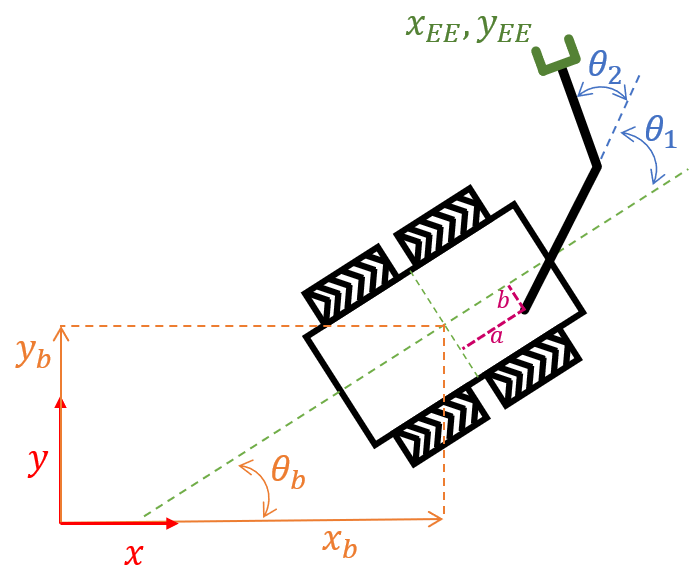
\includegraphics[scale=0.8]{MM_kinematics}
\label{MM_kin}
\caption{A simple Mobile Manipulator composed by a mobile base and a 2-DoF robotic arm}
\end{figure}
Considering the general case of a mobile manipulator composed by a manipulator arm mounted on a mobile platform, its kinematic model set the location of the end effector as a function of both the arm and base generalized coordinates.
\begin{equation}\label{dirkinMM}
	X_{EE}=\left[\begin{matrix}p_{EE}\\\Phi\end{matrix}\right]=f(q)=f\left(\left[\begin{matrix}q_a\\q_b \end{matrix}\right]\right)
\end{equation}
Where $p_{EE}=\left[\begin{matrix}x_{EE}&y_{EE}&z_{EE}\end{matrix}\right]^T$ is the vector of the end effector position and$\Phi =\left[\begin{matrix}\vartheta_{EE}&\varphi_{EE}&\psi_{EE}\end{matrix}\right]$ is the vector of the end effector orientation that can be expressed with different conventions like Azimut-Elevation-Rotation or Roll-Pitch-Yaw.
It is possible to define the function $f$ of Eq.\ref{dirkinMM} adding the rototranslation matrix $A_{base}^{global}$ relative to the mobile base motion, to the direct kinematics of the arm \ref{AAAA}.
\begin{equation}
	A_{base}^{global}=\left[\begin{matrix}
		\cos\theta&-\sin\theta&0&x_b+\sqrt{a^2+b^2}\cos\theta\\
		\sin\theta&\cos\theta&0&y_B+\sqrt{a^2+b^2}\sin\theta\\
		0&0&1&h_{base}\\
		0&0&0&1
	\end{matrix}\right]
\end{equation}
So the forward kinematics can be obtained consequently:
\begin{equation}
A_{ee}^{global}=A_{base}^{global}A_1^{base}A_2^1\cdots A_{ee}^{ee-1}
\end{equation}
Differentiating $f$ we can obtain the differential forward kinematics of the Mobile Manipulator. 
\begin{equation}
	\dot{X}_{EE}=\frac{\partial f}{\partial q_a}(q_a,\theta)\dot{q}_a+\frac{\partial f}{\partial q_b}(q_a,\theta)\dot{q}_b
\end{equation}
Where $\frac{\partial f}{\partial q_a}$ is the same as described in section \ref{jacobians}, and $\frac{\partial f}{\partial q_b}(q_a,\theta)$ can be obtained at the same way considering $x$ and $y$ as prismatic joints and $\theta$ as a revolute joint of the compound system.
In doing this the nonholonomic constraint for the mobile platform should be taken into account:
As we had said before the forward kinematics of a system is always solvable, but for redundant systems like mobile manipulators the inverse kinematics problem has infinite solutions. 
\begin{equation}\label{dynamicsMM}
B\left(q\right)\ddot{q}+C\left(q,\dot{q}\right)\dot{q}+g\left(q\right)=\ \tau
\end{equation}





\subsection{Mixed Kinematics and Dynamics Model}
The idea of the following model is to describe kinematically the mobile base and dynamically the manipulator, in order to have as inputs:
\begin{itemize}\itemsep1pt
	\item[--] the torques applied at the manipulator joints
	\item[--] the longitudinal and angular velocity of the mobile base.
\end{itemize}
For this purpose, the kinematic equation of the mobile base will be used within the dynamic model of the whole mobile manipulator. 
We will notate the variables in the following way.\\
Mobile base coordinates: $x= \left[\begin{matrix}x\\y\\\theta\end{matrix}\right]$\\
Manipulator coordinates: $ q=\left[\begin{matrix}\theta_1\\\theta_2\\\begin{matrix}\vdots\\\theta_6\\\end{matrix}\\\end{matrix}\right]$\\
Vector of longitudinal and angular velocity of the base: $v= \left[\begin{matrix}v_{long}\\\omega\\\end{matrix}\right]$\\
Writing down the dynamic equation of the entire mobile manipulator, which can be obtained as described in section \ref{sec:dynamics}:
\begin{equation}
	B\left(x,q\right)\left[
		\begin{matrix}\ddot{x}\\\ddot{q}\\
	\end{matrix}
	\right]+C\left(x,\dot{x},q,\dot{q}\right)\left[
	\begin{matrix}
		\dot{x}\\\dot{q}\\
	\end{matrix}\right]+g\left(x,q\right)= \left[
	\begin{matrix}
		\tau_x\\\tau_q\\
	\end{matrix}\right]+\left[
	\begin{matrix}
		A(x)\\0\\
	\end{matrix}\right]\lambda
\end{equation}
\begin{equation}
\begin{split}
	\left[
	\begin{matrix}
	B_x(x,q)&B_{xq}(x,q)\\
	B_{qx}(x,q)&B_q(x,q)
	\end{matrix}\right]\left[
	\begin{matrix}
	\ddot{x}\\\ddot{q}
	\end{matrix}\right]&\\ +\left[
	\begin{matrix}
	C_x(x,\dot{x},q,\dot{q})&C_{xq}(x,\dot{x},q,\dot{q})\\
	C_{qx}(x,\dot{x},q,\dot{q})&C_q(x,\dot{x},q,\dot{q})
	\end{matrix}\right]\left[
	\begin{matrix}
	\dot{x}\\\dot{q}
	\end{matrix}\right] &\\ +\left[
	\begin{matrix}
	0\\g(q)
	\end{matrix}\right]	&= \left[
	\begin{matrix}
	\tau_x\\\tau_q\\
	\end{matrix}\right]+\left[
	\begin{matrix}
	A(x)\\0\\
	\end{matrix}\right]\lambda
\end{split}	
\end{equation}
Premultiplying by $G^T$ only the rows relative to the base coordinates:
\begin{equation}
\begin{split}
	\left[\begin{matrix}G^T(x)B_x(x,q)&G^T(x)B_{xq}(x,q)\\B_{qx}(x,q)&B_q(x,q)\\\end{matrix}\right]\left[\begin{matrix}\ddot{x}\\\ddot{q}\\\end{matrix}\right] &\\
	+\left[\begin{matrix}G^T(x)C_x(x,\dot{x},q,\dot{q})&G^T(x)C_{xq}(x,\dot{x},q,\dot{q})\\C_{qx}(x,\dot{x},q,\dot{q})&C_q(x,\dot{x},q,\dot{q})\\\end{matrix}\right]\left[\begin{matrix}\dot{x}\\\dot{q}\\\end{matrix}\right] &\\
	+\left[\begin{matrix}0\\g(q)\\\end{matrix}\right]
	&= \left[\begin{matrix}G^T(x)\tau_x\\\tau_q\\\end{matrix}\right]
\end{split}
\end{equation}

The columns of $G$ are a basis of the null space of $A(x)T$, so the Lagrange multipliers term is set to zero.
If we now consider the kinematic equation of the base \ref{G}:
\begin{equation}
	\left[\begin{matrix}\dot{x}\\\dot{q}\\\end{matrix}\right]=\left[\begin{matrix}G(x)&0\\0&I\\\end{matrix}\right]\left[\begin{matrix}v\\\dot{q}\\\end{matrix}\right]
	\end{equation}
Whose derivative is:
\begin{equation}
	\ddot{x}=G\left(x\right)\dot{v}+\dot{G}\left(\dot{x},x\right)v
\end{equation}
\begin{equation}
	\left[\begin{matrix}\ddot{x}\\\ddot{q}\\\end{matrix}\right]=\left[\begin{matrix}G(x)&0\\0&I\\\end{matrix}\right]\left[\begin{matrix}\dot{v}\\\ddot{q}\\\end{matrix}\right]+\left[\begin{matrix}\dot{G}\left(\dot{x},x\right)&0\\0&0\\\end{matrix}\right]\left[\begin{matrix}v\\\dot{q}\\\end{matrix}\right]
\end{equation}
If we substitute these expressions in the dynamic model of the mobile manipulator:
\begin{equation} \label{kinodyn}
	\left[\begin{matrix}G^TB_xG&G^TB_{xq}\\B_{qx}G&B_q\\\end{matrix}\right]\left[\begin{matrix}\dot{v}\\\ddot{q}\\\end{matrix}\right]+\left[\begin{matrix}G^TB_x\dot{G}+G^TC_xG&G^TC_{xq}\\B_{qx}\dot{G}+C_{qx}G&C_q\\\end{matrix}\right]\left[\begin{matrix}v\\\dot{q}\\\end{matrix}\right]+\left[\begin{matrix}0\\g\\\end{matrix}\right]=\ \left[\begin{matrix}G^T\tau_x\\\tau_q\\\end{matrix}\right]
\end{equation}
Where the parenthesis have not been transcribed in order to have a compact expression.
What now we are interested in is the dynamic equation of only the manipulator part, i.e. the second row of \ref{kinodyn}.
\begin{equation}
	\left[\begin{matrix}B_{qx}G&B_q\\\end{matrix}\right]\left[\begin{matrix}\dot{v}\\\ddot{q}\\\end{matrix}\right]+\left[\begin{matrix}B_{qx}\dot{G}+C_{qx}G&C_q\\\end{matrix}\right]\left[\begin{matrix}v\\\dot{q}\\\end{matrix}\right]+g=\ \tau_q
\end{equation}
$v$, which is the velocity vector of the base, is the input vector of the kinematic model of the base. The idea is to use $v$ and $\dot{v}$ as inputs also in the dynamic model of the manipulator. 
Rearranging the previous equation we obtain:
\begin{equation}
	\left[B_q\right]\ddot{q}+\left[C_q\right]\dot{q}+g=\ \tau_q-\left[B_{qx}G\right]\dot{v}-\left[B_{qx}\dot{G}+C_{qx}G\right]v
\end{equation}
Which in state space form is:
\begin{equation}
\begin{split}
	\left[\begin{matrix}\ddot{q}\\\dot{q}\\\end{matrix}\right]&=\left[\begin{matrix}-{B_q}^{-1}C_q&0\\I&0\\\end{matrix}\right]\left[\begin{matrix}\dot{q}\\q\\\end{matrix}\right]+\left[\begin{matrix}{{-B}_q}^{-1}g\\0\\\end{matrix}\right]+\left[\begin{matrix}{B_q}^{-1}\\0\\\end{matrix}\right]\tau_q\\&+\left[\begin{matrix}-{B_q}^{-1}B_{qx}G\\0\\\end{matrix}\right]\dot{v}\\&+\left[\begin{matrix}-{B_q}^{-1}\left[B_{qx}\dot{G}+C_{qx}G\right]\\0\\\end{matrix}\right]v
\end{split}
\end{equation}
Adding also the kinematic equation of the base we have the entire model of the system in state space form:
\begin{equation}
	\begin{split}
		\left[\begin{matrix}\ddot{q}\\\dot{q}\\\dot{x}\\\end{matrix}\right]&=\left[\begin{matrix}-{B_q}^{-1}C_q&0&0\\I&0&0\\0&0&0\\\end{matrix}\right]\left[\begin{matrix}\dot{q}\\q\\x\\\end{matrix}\right]+\left[\begin{matrix}{{-B}_q}^{-1}g\\0\\0\\\end{matrix}\right]+\left[\begin{matrix}{B_q}^{-1}\\0\\0\\\end{matrix}\right]\tau_q\\&+\left[\begin{matrix}-{B_q}^{-1}B_{qx}G\\0\\0\\\end{matrix}\right]\dot{v}\\&+\left[\begin{matrix}-{B_q}^{-1}\left[B_{qx}\dot{G}+C_{qx}G\right]\\0\\G\\\end{matrix}\right]v 
	\end{split}
\end{equation}
More precisely:
\begin{equation}
	\begin{split}
			\left[\begin{matrix}\ddot{q}\\\dot{q}\\\dot{x}\\\end{matrix}\right]&=\left[\begin{matrix}-{B_q}^{-1}(x,q)C_q(x,\dot{x},q,\dot{q})&0&0\\I&0&0\\0&0&0\\\end{matrix}\right]\left[\begin{matrix}\dot{q}\\q\\x\\\end{matrix}\right]+\left[\begin{matrix}{{-B}_q(x,q)}^{-1}g(q)\\0\\0\\\end{matrix}\right]\\&+\left[\begin{matrix}{B_q(x,q)}^{-1}\\0\\0\\\end{matrix}\right]\tau_q\\&+\left[\begin{matrix}-{B_q(x,q)}^{-1}B_{qx}(x,q)G(x)\\0\\0\\\end{matrix}\right]\dot{v}\\&+\left[\begin{matrix}-{B_q(x,q)}^{-1}\left[B_{qx}(x,q)\dot{G(x)}+C_{qx}(x,\dot{x},q,\dot{q})G(x)\right]\\0\\G(x)\\\end{matrix}\right]v 
	\end{split}
\end{equation}


